\chapter{The QT communication potential on Twitter} 
Lorem ipsum dolor sit amet, consectetur adipisci elit, sed eiusmod tempor incidunt ut labore et dolore magna aliqua. Ut enim ad minim veniam, quis nostrum exercitationem ullam corporis suscipit laboriosam, nisi ut aliquid ex ea commodi consequatur. Quis aute iure reprehenderit in voluptate velit esse cillum dolore eu fugiat nulla pariatur. Excepteur sint obcaecat cupiditat non proident, sunt in culpa qui officia deserunt mollit anim id est laborum.

Data shown in this chapter was collected with the Twitter Analytics Tool Twitonomy. 

\section{Hashtag performance}
Two hashtags were monitored to assess of the reach potential of FET projects on QTs. These were \#quantumcomputing and the application of the AND logic operator to \#quantum and \#technology. 

Both analyses covered two periods of time. For \#quantumcomputing, the two periods were from 7th to 14th and from 20th to 25th October 2017, respectively. Those for the combination \#quantum AND \#technology spanned the time intervals between 4th and 14th and between 15th and 25th October 2017. The time periods were chosen randomly and based on the day ranges available to Twitonomy for the considered volume of tweets. Different choices of the time periods would not change significantly the estimates presented in this chapter.  

The distribution of the number of Tweets presenting the hashtags \#quantumcomputing and the combination \#quantum AND \#technology over the considered periods are shown in figures \ref{First-SecondSearch_QuantumComputing.png} and \ref{First-SecondSearch_QuantumTechnology.png}. The plots show that, typically, hundreds of tweets with the hashtag \#quantumcomputing are posted daily, whereas few show both hashtags \#quantum and \#technology. 

The potential reach of FET projects on QTs is summarised by data in Tables \ref{Summary_QuantumComputing-Technology}. 

\begin{table}[t]
 \begin{center}
 
  \begin{tabular}{ccccc}
   \hline 
   \hline
   Time period & Tweets & Users & Potential Reach \\ 
   \hline
   \hline
   7 - 14 Oct 2017 & 1 928 & 1 270 & 9 392 166  \\
   20 - 25 Oct 2017 & 2 563 & 1 738 & 10 604 445  \\
   \hline
   \hline
  \end{tabular}

  \bigskip

  \begin{tabular}{ccccc}
   \hline 
   \hline
   Time period & Tweets & Users & Potential Reach \\ 
   \hline
   \hline
   4 - 14 Oct 2017 & 79 & 75 & 280 849  \\
   15 - 25 Oct 2017 & 36 & 28 & 85 123  \\
   \hline
   \hline
  \end{tabular}
 \end{center} 
 \caption{Summary of the Twitter analytics for the hashtag combination \#quantum AND \#technology over the two monitored time periods. The potential reach is defined as the total aggregate number of followers of the people who mentioned the considered keyword in their tweets.}
\label{Summary_QuantumComputing-Technology} 
\end{table}    

\begin{figure}
 \centering
 \begin{subfigure}[b]{0.9\textwidth}
   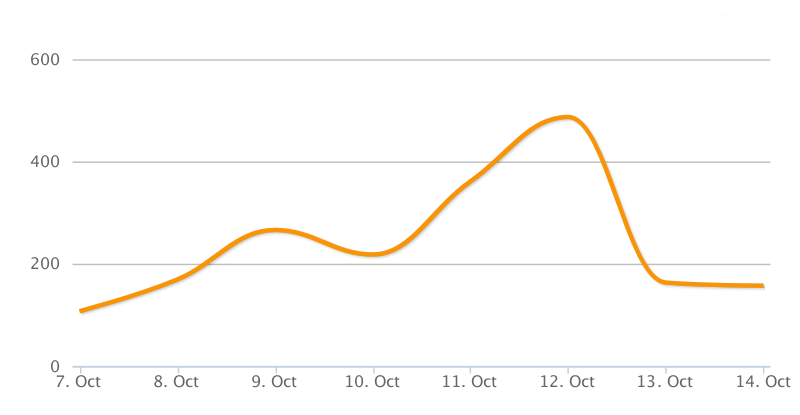
\includegraphics[width=1\linewidth]{Images/FirstSearch_QuantumComputing.png}
   \caption{} 
 \end{subfigure}

 \begin{subfigure}[b]{0.9\textwidth}
   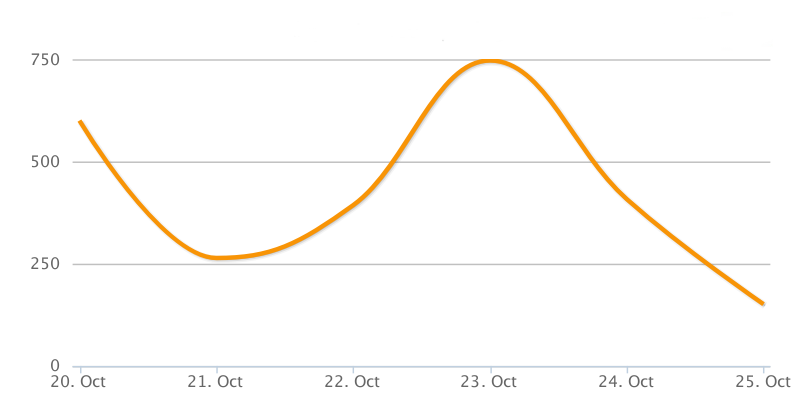
\includegraphics[width=1\linewidth]{Images/SecondSearch_QuantumComputing.png}
   \caption{}
 \end{subfigure}
 \caption{(a) Number of tweets with hashtag \#quantumcomputing posted between 7th and 14th October 2017. (b) As for (a) but over the time period between 20th and 25th October 2017.} 
 \label{First-SecondSearch_QuantumComputing.png}
\end{figure}

\begin{figure}
 \centering
 \begin{subfigure}[b]{0.9\textwidth}
   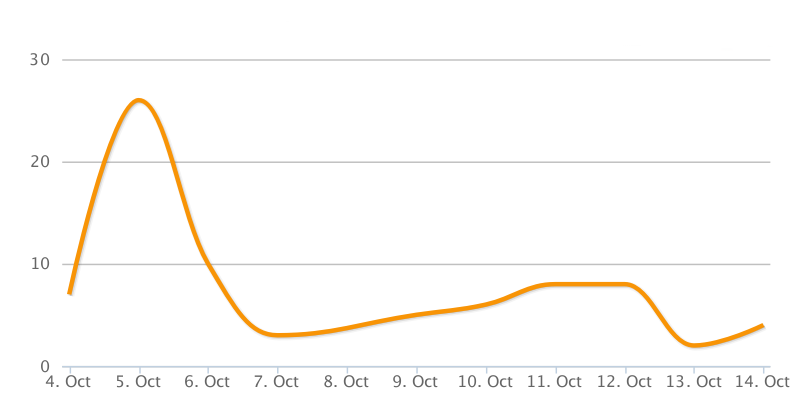
\includegraphics[width=1\linewidth]{Images/FirstSearch_QuantumTechnology.png}
   \caption{} 
 \end{subfigure}

 \begin{subfigure}[b]{0.9\textwidth}
   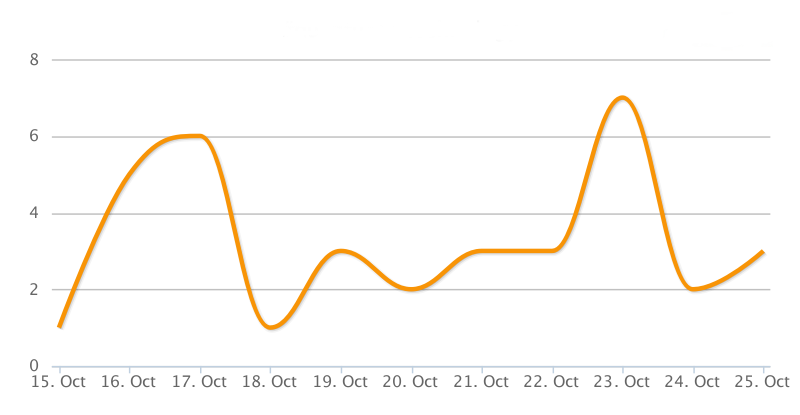
\includegraphics[width=1\linewidth]{Images/SecondSearch_QuantumTechnology.png}
   \caption{}
 \end{subfigure}
 \caption{(a) Number of tweets with hashtags \#quantum and \#technology posted between 4th and 14th October 2017. (b) As for (a) but over the time period between 15th and 25th October 2017.} 
 \label{First-SecondSearch_QuantumTechnology.png}
\end{figure}